\documentclass[norsk,a4paper,12pt]{article}
\usepackage[utf8]{inputenc}
\usepackage[T1]{fontenc} %for å bruke æøå
\usepackage[utf8]{inputenc}
\usepackage{graphicx} %for å inkludere grafikk
\usepackage{verbatim} %for å inkludere filer med tegn LaTeX ikke liker
\usepackage{mathpazo}
\usepackage{amsmath}
\usepackage{float}
\usepackage{amsmath}
\usepackage{hyperref}
\newcommand\numberthis{\addtocounter{equation}{1}\tag{\theequation}}
\bibliographystyle{plain}

\begin{document}
\title{FYS3150-Project 1}
\author{Marcus Berget, Sebastian Amundsen, Andreas Wetzel}
\date{August 2020}
\maketitle

\begin{abstract}
We have compared three methods of solving a discretized version of one dimensional Poisson equation with Dirichlet  conditions. These three methods include using two different algorithms exploiting that the second derivative takes form of a tri-diagonal matrix. The third method is using LU-decomposition. The algorithm for our specific case has the least amount of floating point operations and fastest run-time, with the LU-decomposition method being the slowest with the largest amount of floating point operations. 
\end{abstract}

\section{Introduction}

In this project we will use numerical methods to solve the one dimensional Poisson equation with Dirichlet boundary conditions. We will be rewriting the equation as a set of linear equations. Our numerical methods will have varying degrees of accuracy. We are going to compare our algorithms and the CPU time for the different numerical methods. 

\section{Method}
The one dimensional Poisson equation with Dirichlet boundary conditions is given by:

\begin{equation}
-u''(x)=f(x) \hspace{1cm} x \in (0,1) \hspace{1cm} u(0)=u(1)=0
 \label{eq:udd}
 \end{equation}

Let's define the discretized approximation to $u(x)$ as $v_i$, and to $f(x)$ as $f_i$. We can then make an approximation of the second derivative of $u$ given by:

\begin{equation}
\frac{-v_{i+1}+v_{i-1}-2v_i}{h^2}=f_i, \textrm{  where  } i=1,2,3......,n,
 \label{eq:2der}
 \end{equation}
 
 Here the step length of spacing is given by $h=1/(n+1)$ and the grid points are defined by $x_i=ih$. We can then rewrite equation (\ref{eq:2der}) as a linear set of equations on the form $\textbf{A}\textbf{v}=\tilde{\textbf{b}}$:
\begin{align*}
\textbf{A}\textbf{v}&= \begin{bmatrix} 2 & -1 & 0 & \dots & \dots & 0 \\ -1 & 2 & -1 & 0 & \dots & \dots \\ 0 & -1 & 2 & -1 & 0 & \dots \\ \vdots & \vdots & \vdots & \ddots \\ 0 & \vdots & \vdots & -1 & 2 & -1 \\ 0 & \vdots & \vdots & 0 & -1 & 2  \end{bmatrix}
\begin{bmatrix} v_0 \\ v_1\\ v_2\\ \vdots \\ v_n \\ v_{n+1} \end{bmatrix}=\begin{bmatrix} 2v_0 - v_1 \\ -v_0+2v_1-v_2 \\ -v_1+2v_2-v_3 \\ \vdots \\ -v_{n-1}+2v_n-v_{n+1} \\ -v_n+2v_{n+1}
\end{bmatrix}\\ &=
\begin{bmatrix}h^2f_0 \\ h^2f_1\\ h^2f_2\\ \vdots \\ h^2f_n\\ h^2f_{n+1}\end{bmatrix} = \widetilde{\textbf{b}} \numberthis \label{eq:lineq}
\end{align*}

In our case we will use the source term $f(x)=100e^{-10x}$ which gives us a closed form solution $u(x)$ given by:

\begin{equation}
u(x)=1-(1-e^{-10})x-e^{-10x}
\label{eq:d_i}
\end{equation}

We will use this solution as a point of reference to discuss the accuracy of our numerical methods. 

\subsection{General algorithm for tri-diagonal matrix}

There exists an algorithm for solving generic sets of linear equations, but in the case for equation (\ref{eq:lineq})  where we have a tri-diagonal matrix we can use a different algorithm which decreases the amount of floating point operations needed. We denote the elements in the leading diagonal of A as $b_1, b_2, ..., b_n$, the elements above the leading diagonal as $a_2, a_3 ..., a_n$, and the elements below the leading diagonal as $c_1, c_2, ..., c_{n-1}$. The algorithm uses a forward substitution to replace the leading diagonal with elements denoted by $\tilde{b}_i$, and replaces the righthand side in with the elements $\tilde{f}_i$ as shown below:
\begin{align*}
\tilde{b}_i=b_i-\frac{a_ic_{i-1}}{\tilde{b}_{i-1}} \\
\tilde{f}_i=f_i-\frac{a_i\tilde{f}_{i-1}}{\tilde{b}_{i-1}}
\end{align*}
where $\tilde{b}_1=b_1$ and $\tilde{f}_i=f_i$. The algorithm then continues with a backward substitution which gives the solution:
\begin{align}
u_{i-1}=\frac{\tilde{f}_{i-1}-c_{i-1}u_i}{\tilde{b}_{i-1}}
\end{align}
\\
\subsection{Algorithm for specific tri-diagonal matrix}

In our special case we can implement a solver that is even simpler than what is described previously.  We will exploit the fact that the matrix has identical matrix elements along the diagonal and identical values for the non diagonal elements $\vec{e}_i$. In this case we can precalculate the new values for the updated matrix elements $d_i$ without taking into account the values for $\vec{e}_i$:

\begin{equation}
d_i = 2-\frac{1}{\tilde{d}_{i-1}}=\frac{i+1}{i}
 \label{eq:d_i}
 \end{equation}

Here the initial value is $\tilde{d}_1=2$. The new righthand side solution $\tilde{f}_i$ is given by:

\begin{equation}
\tilde{f}_i = f_i + \frac{(i-1)\tilde{f}_{i-1}}{i}
 \label{eq:f_i}
 \end{equation}

Here the initial value is $\tilde{f}_1=f_1$. The last step is to make a backward substitution which gives the final solution $u_i$:

\begin{equation}
u_{i-1}=\frac{i-1}{i}(\tilde{f}_{i-1}+\tilde{u})
 \label{eq:u_i-1}
 \end{equation}
 
 This method requires that we know the last value $u_n$ in the $u_i$ array. This value is given by $u_n=\tilde{f}_n/\tilde{b}_n$. 
 
 \subsection{Relative error}
 
 Algorithms have a varying degree of uncertainty. We will test how precise our algorithm is for the specific tri-diagonal matrix case. The numerical solution will be compared to the analytical solution given the relative error $\epsilon_i$:
 
 \begin{equation}
\epsilon_i = \log_{10}\bigg(\bigg|\frac{v_i-u_i}{u_i}\bigg|\bigg)
 \label{eq:eps}
 \end{equation}
 
For the numerical $v_i$ and analytical $u_i$ function values. We wish to extract the max value of the relative error for varying numbers of grid points n. This will give us some information about how precise the numerical approximation is compared to the analytical solution.

 \subsection{LU decomposition}

We are now going to LU factorize the matrices 10 x 10, 100 x 100, 1000 x 1000 and 10 000 x 10 000. What the LU decomposition does, is that it rewrites a matrix as the product of two other matrices L and U, like this:
\begin{align*}
\begin{bmatrix}
a_{11} & a_{12} & .... & a_{1n} \\
a_{21} & a_{22} & .... & a_{2n} \\
: & :& .... & : \\
a_{n1} & a_{n2} & .... & a_{nn} \\
\end{bmatrix}
=
\begin{bmatrix}
1 & 0 & .... & 0 \\
l_{21} & 1 & .... & 0 \\
: & :& .... & : \\
l_{n1} & l_{n2} & .... & 1\\
\end{bmatrix}
\begin{bmatrix}
u_{11} & u_{12} & .... & u_{1n} \\
0 & u_{22} & .... & u_{2n} \\
: & :& .... & : \\
0 & 0& .... & u_{nn} \\
\end{bmatrix}
\end{align*}  
\\
\\
In order to calculate a set of linear equation by using the LU decomposition for matrix Ax=w. We first need to compose a matrix A of two matrices L and U. When we have done that we split our equation in to two equation:
\\
\\
\begin{align*}
\mathbf{A}\mathbf{x}=\mathbf{L}\mathbf{U}\mathbf{x}=\mathbf{b}\\
\mathbf{A}\mathbf{x}=\mathbf{L}\mathbf{U}\mathbf{x}=\mathbf{b}\\
\mathbf{L}\mathbf{y}=\mathbf{b} \land  \mathbf{U}\mathbf{x}=\mathbf{y}\\
\end{align*}
\begin{align*}
\end{align*}
Where $\mathbf{b}$ is given as the one-dimensional Poisson equation times the square of the step length h. $$\mathbf{b}=-\frac{d^2u}{dx^2}h^2=f(x)h^2$$
Since we now have obtained two separated equation, we now solve for y in equation $$\mathbf{L}\mathbf{y}=\mathbf{b} \rightarrow \mathbf{L}\mathbf{y}=\mathbf{b} $$ Which we afterwards plug in  $$\mathbf{U}\mathbf{x}=\mathbf{y} \rightarrow \mathbf{x}=\mathbf{U^{-1}}\mathbf{y}$$, which then gives us vector $\mathbf{x}$.

\section{Implementation}

All programs used is available at: \\
\url{https://github.com/Sebamun/FYS3150_Projekter}

We implement the algorithms numerically with varying values of grid points n. The approximations are plotted for the general algorithm and we find the relative error for the specific case. The relative error is really high at the endpoints for the specific algorithm. This is due to the ratio between numerator and denominator in equation \ref{eq:eps}. This is solved by excluding the endpoints for the approximation. 

\section{Results}

\subsection{General algorithm}

\begin{figure}[H]
	\centering
	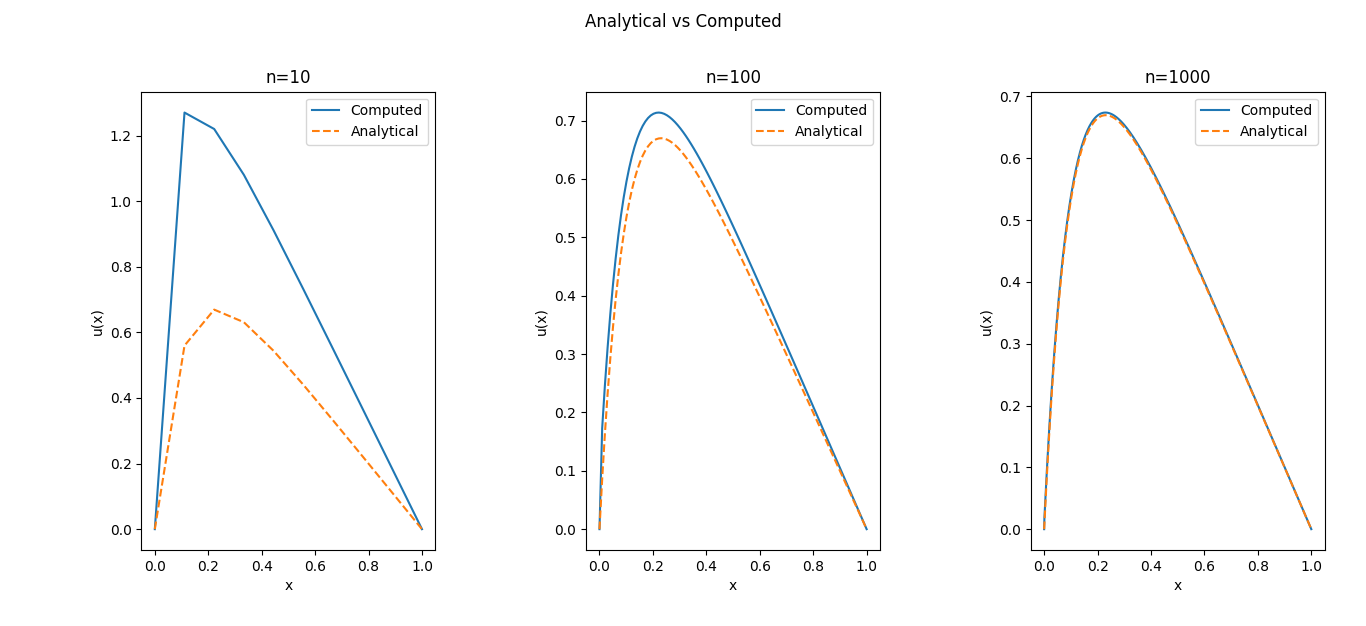
\includegraphics[width=\linewidth]{1b.png}
	\caption{Plot comparing analytical vs computed solutions of the differential equation. We can see that the computed solution approaches the analytical solution when the number of gridpoints increases.}
	\label{fig:1bplot}
\end{figure}

We found that the number of floating point operations are 9 per iteration for the general algorithm. The CPU time is given in Table (\ref{tab:LU}).

\subsection{Algorithm for specific tri-diagonal matrix}

We found that the number of floating point operations are 4 per iteration for the general algorithm. The CPU time is given in Table (\ref{tab:LU}).

 \subsection{Relative error}
 
  \begin{table}[H]
\begin{center}
\caption{Relative error for specific tri-diagonal matrix algorithm.}
\begin{tabular}{ |c|c|c| } \hline
Steps (n)&Relative error ($\epsilon$) \\ \hline
$10$&$6.20*10^{-1}$ \\ \hline
$10^2$&$1.21*10^{-1}$ \\ \hline
$10^3$&$2.36*10^{-2}$ \\ \hline
$10^4$&$3.61*10^{-3}$ \\ \hline
$10^5$&$4.89*10^{-4}$ \\ \hline
$10^6$&$6.17*10^{-5}$ \\ \hline
$10^7$&$7.45*10^{-6}$ \\ \hline
\end{tabular}
\label{tab:e}
\end{center}
\end{table}

 \subsection{LU decomposition}
 
   \begin{table}[H]
\begin{center}
\caption{CPU time of algorithms.}
\begin{tabular}{ |c|c|c|clcl } \hline
Size & Generel algorithm& Special algorithm& LU decomposition \\ \hline
n =10 & 0.0002 seconds &0.0002 seconds&0.585 seconds\\ \hline
n = 100 & 0.0007 seconds   &0.0005  seconds& 0.591 seconds\\ \hline
n = 1000 &0.0041 seconds &0.003 seconds& 0.736 seconds\\ \hline
n = 10 000    &0.0336 seconds&0.0245  seconds&56.580 seconds\\ \hline
n = 100 000& 0.306 seconds &0.233 seconds& ...\\ \hline
n = 1 000 000 & 3.011 secondss &2.245 seconds&...\\ \hline
\end{tabular}
\label{tab:LU}
\end{center}
\end{table}

The number of floating point operations for the LU decomposition is $\frac{2}{3} n^3$.

\section{Discussion}

The number of floating point operations are different for each of our algorithms. Our algorithm for the specific tri diagonal matrix has the least amount of floating point operations. In practice this means that the CPU time should be less for the specific case than for the general algorithm and the LU method. Our time tests show this exact trend (Table \ref{tab:LU}). The LU method have the highest amount of FLOPS, which leads to it being the slowest method for our matrix. FLOPS depend on the size of the matrix. When the matrix becomes large in our LU method, we can ignore the orders $n$ and $n^2$.     

We can see from table \ref{tab:e} that the relative error decreases as n increases. This is due to the fact that more grid points lead to better precision. However this is only true up to a certain point. If we would increase the number of grid points further our relative error could potentially increase dramatically. This is due to the fact that by using more grid points we could encounter round off errors which in turn would make the computed relative error very large. Since we are using python, more than $n=10^7$ grid points make the algorithm take too long to run. We could have used a larger n If we had used a faster programming language (like C++), making it possible to observe an increasing relative error at a larger n.

If we compare our solution from the general algorithm and the CPU-time for the LU decomposition (Table \ref{tab:e}), we see that it takes a lot of more time to calculate the LU decomposition. This is due to the fact that it takes $n^3$ steps to find the LU decomposition (which is the same as for the gaussian- elimination method). The advantage of using LU decomposition is that it can be used to solve multiple different vectors, with one less calculation than for the gaussian elimination method. The remaining calculation only takes $n^2$ floating point operations. This can save a lot of time if you wish to solve multiple vectors with the same matrix. In our case the LU decompositions is essentially unnecessary since we only solve one vector per matrix. Another benefit of the LU decomposition is that it makes it straight forward to solve the determinant of a matrix.

The reason why we can’t use LU decomposition on a $10^5 \times 10^5$ matrix is due to a random accesses memory problem. The data that needs be stored for this operation is too large for the computers memory. 

\section{Concluding remarks}
We have compared three methods of solving the one dimensional Poisson equation with Dirichlet  conditions. The method where we used the specific algorithm for tri-diagonal matrices has the fastest run-time and uses the least amount of RAM. The disadvantage of using this method is that it only applies to matrices with identical elements along the diagonals. However, using the algorithm for generic trio-diagonal matrices is not much slower than using the specific algorithm, at least compared to the LU-decomposition method which by far is the slowest. So when choosing an algorithm for solving similar problems, finding a viable algorithm with the least amount of floating point operations should be high on your priority list. 
\bibliography{referanser}
http://compphysics.github.io/ComputationalPhysics/doc/pub/linalg/pdf/linalg-print.pdf
\end{document}
